\chapter{Introduction}
\label{ch:Introduction}

\section{General}

Human body motion analysis has become an integral part of medical diagnostic techniques. 

\section{Goals}

The goal of this thesis was implementing a new Kalman filter based orientation algorithm proposed by \citeauthor{bennett_motion_2014} in \cite{bennett_motion_2014} to improve the estimation of orientation angles by means of inertial sensors.

\section{Motivation}


\section{GaitWatch}

This paragraph will describe the hardware we used..

The GaitWatch device \cite{olivares_vicente_gaitwatch_2013} is a MIMU designed to monitor the motion of patients while attached to the body. It was developed at the Department of Neurology of the Ludwig-Maximilians University in Munich, Germany, in association with the Department of Signal Theory, Telematics and Communications of the University of Granada, Spain. The system is composed of a set of embedded magnetic and inertial sensors wired to a box containing a microcontroller. This microcontroller is in charge of collecting data from the embedded box sensors, as well as from the external measurement units, and storing them on a memory card. The various units are placed at the patient's trunk, arms, thighs, and shanks as shown in Figure \ref{fig:GaitWatch_placement}. The components of the three different kinds of subunits are described below:


\begin{itemize}

\item \textsc{Type A} -- thighs and shanks: 

IMU Analog Combo Board with 5 Degrees of Freedom \cite{IMU5}, containing an IDG500 biaxial gyroscope, from which only y-axis is actually used, with a measurement range of ±500\,°/s \cite{IDG500} and a ±3\,g triaxial accelerometer, ADXL335 \cite{ADXL335}.

\item \textsc{Type B} -- arms:

IDG500 biaxial gyroscope with a measurement range of ±500\,°/s \cite{IDG500}.

\item \textsc{Type C} -- trunk:

ADXL345 triaxial accelerometer with a programmable measurement range of ±2/±4/±8/±16\,g \cite{ADXL345},
IMU3000 triaxial gyroscope with a programmable measurement range of ±250/±500/±1000/±3000°/s \cite{IMU3000}, 
Micromag3 \allowbreak triaxial magnetometer with a measurement range of ±11\,Gauss \cite{MicroMag3}, AL-XAVRB board containing an AVR ATxmega processor \cite{AVRATxmega}.

\end{itemize}

\begin{figure}
	\centering
	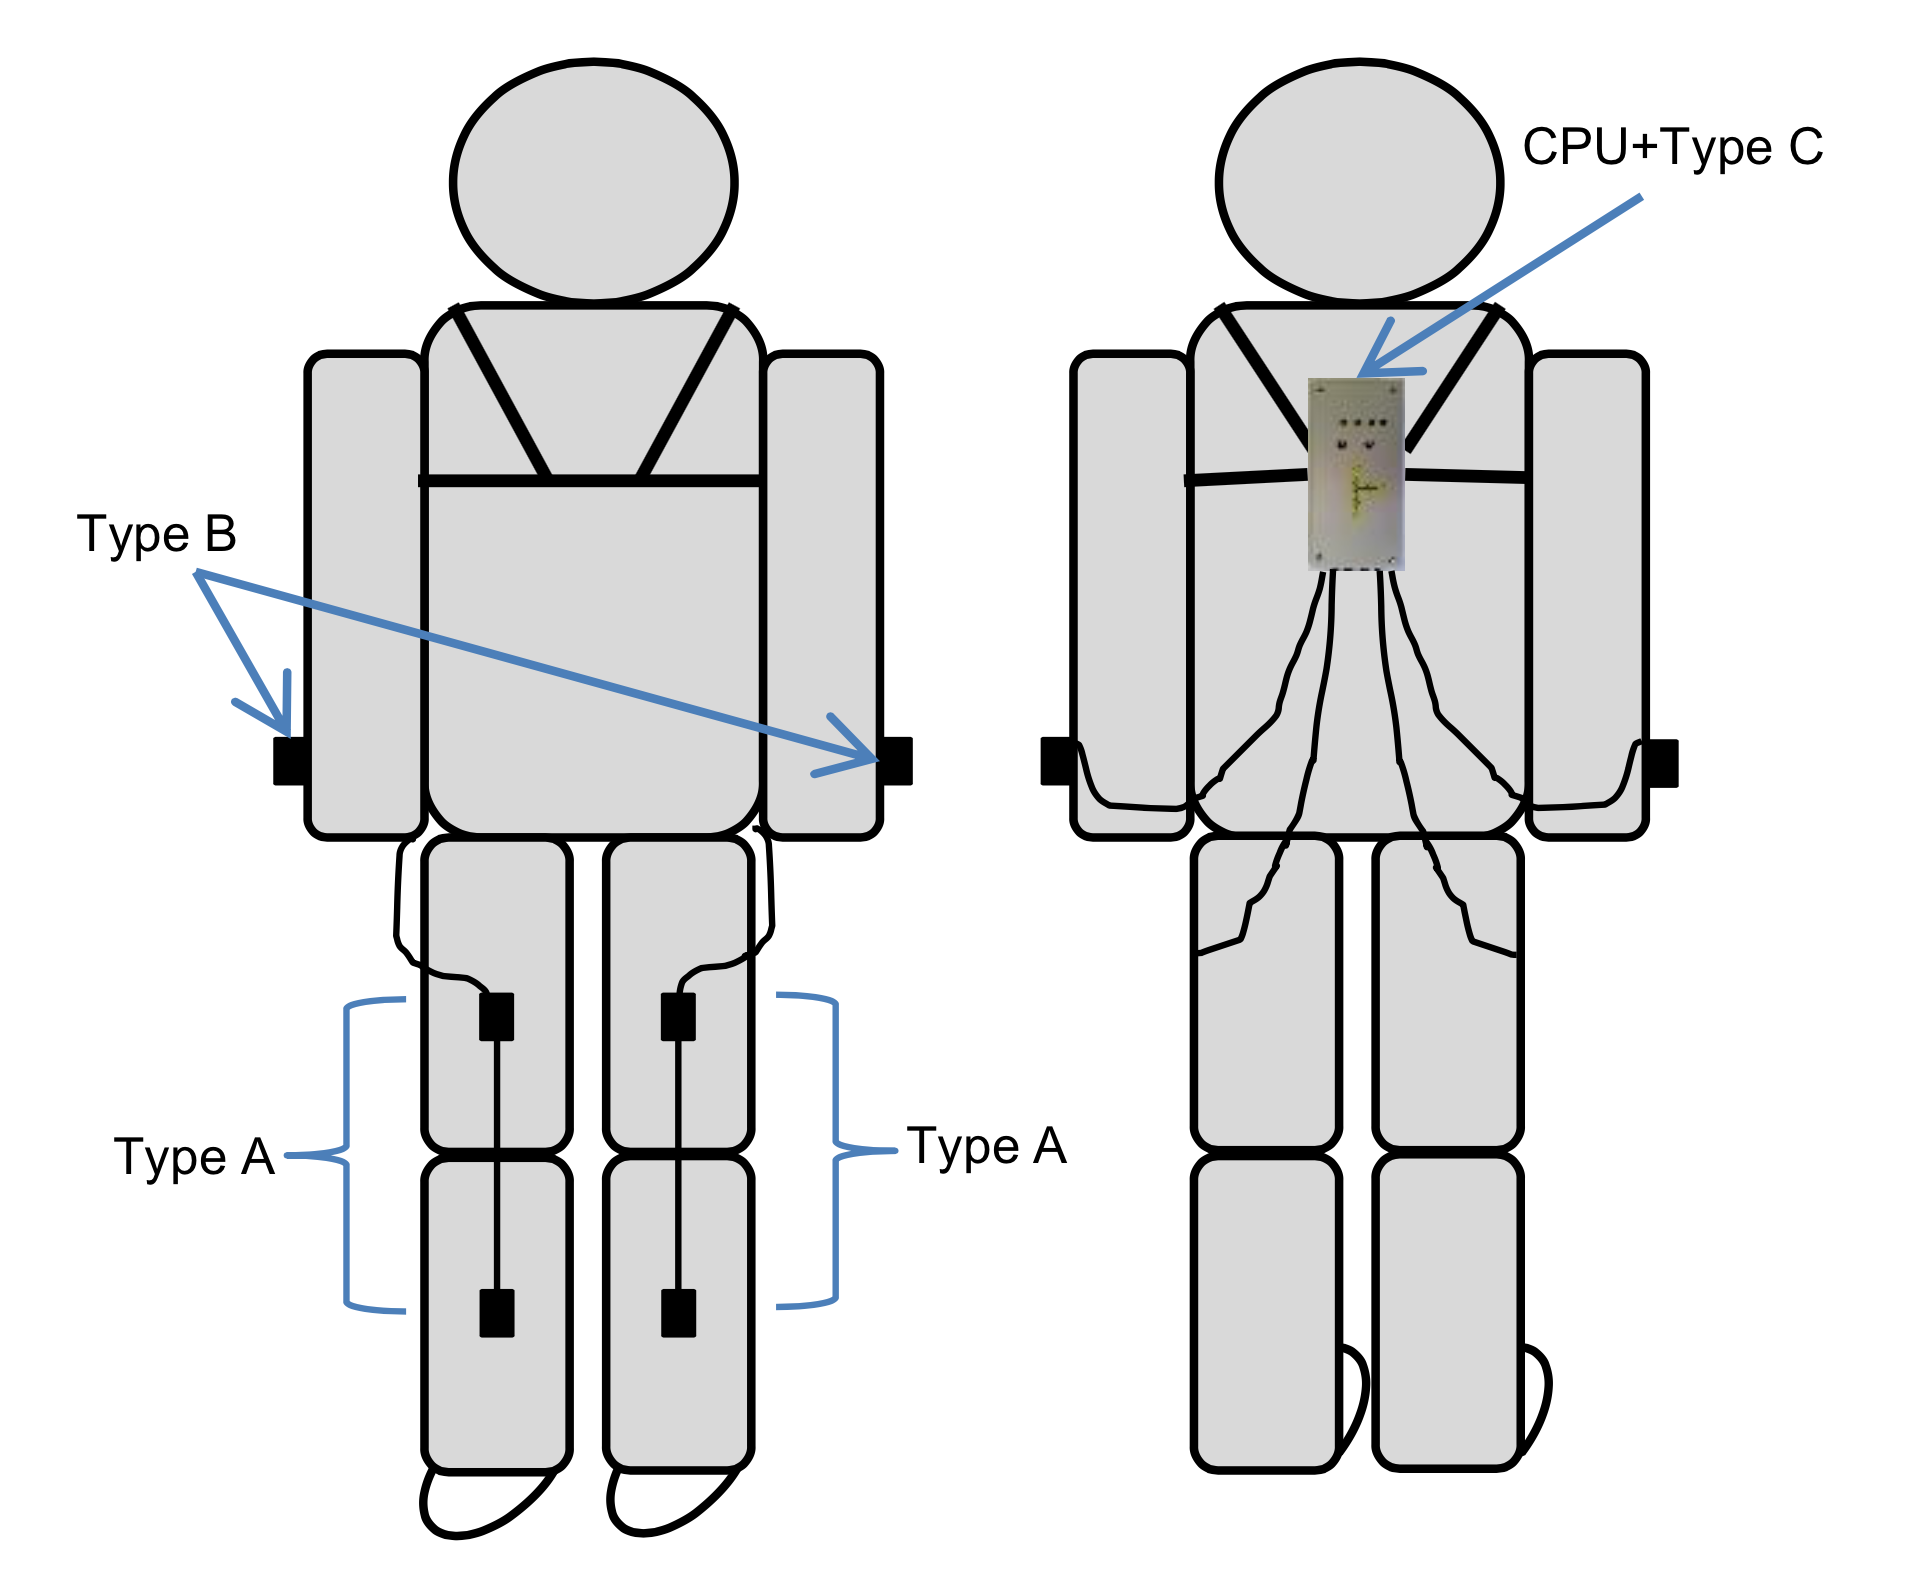
\epsfig{file=images/GaitWatch_placement, width=9cm}
	\caption{Placement of GaitWatch components at the body \cite{olivares_vicente_gaitwatch_2013}.}
	\label{fig:GaitWatch_placement}
\end{figure}

\section{Methodology}

Our Team was composed of three members and worked using the agile software development methodology. Working software was delivered frequently and was the principal measure of progression. To follow the progress of other team members at any time we used Pivotal Tracker, a tool for agile project management and GitHub, a repository hosting service based on the distributed version control system Git. I used the document markup language \LaTeX{} to write this thesis.

\section{Document Structure}

This thesis begins with an introductory chapter where the scope of the concrete task is discussed as well as its goals and ends with the hardware we used. Chapter 2 describes the state of the art. In Chapter 3, we will elaborate on the Fundamentals necessary for the implementation. Chapter 4 presents and discusses the results. Finally, Chapter 5 concludes and proposes possible future work.